\documentclass[12pt]{report}
\usepackage{scribe,graphicx,graphics}
\usepackage{proba}
\usepackage{float}
\usepackage{cancel}
\usepackage{listings}
\newcommand{\norm}[1]{\left|\left|#1\right|\right|}
\usepackage{listings}
\usepackage{xcolor}
\usepackage{listings}
\DeclareMathOperator*{\Tr}{Tr}
\definecolor{codegreen}{rgb}{0,0.6,0}
\definecolor{codegray}{rgb}{0.5,0.5,0.5}
\definecolor{codepurple}{rgb}{0.58,0,0.82}
\definecolor{backcolour}{rgb}{0.95,0.95,0.92}

\lstdefinestyle{mystyle}{
    backgroundcolor=\color{backcolour},   
    commentstyle=\color{codegreen},
    keywordstyle=\color{magenta},
    numberstyle=\tiny\color{codegray},
    stringstyle=\color{codepurple},
    basicstyle=\ttfamily\footnotesize,
    breakatwhitespace=false,         
    breaklines=true,                 
    captionpos=b,                    
    keepspaces=true,                 
    numbers=left,                    
    numbersep=5pt,                  
    showspaces=false,                
    showstringspaces=false,
    showtabs=false,                  
    tabsize=2
}

\lstset{style=mystyle}
\course{CSE 382M} 	
\coursetitle{Found. Data Science \& ML}	
\semester{Spring 2025}
\lecturer{} % Due Date: {\bf Mon, Oct 3 2016}}
\lecturetitle{Problem Set}
\lecturenumber{2}   
\lecturedate{}    
\usepackage{enumerate}
\newcommand{\remind}[1]{\textcolor{red}{\textbf{#1}}} %To remind me of unfinished work to fix later
\newcommand{\hide}[1]{} %To hide large blocks of code without using % symbols

\newcommand{\ep}{\varepsilon}
\newcommand{\vp}{\varphi}
\newcommand{\lam}{\lambda}
\newcommand{\Lam}{\Lambda}
%\newcommand{\abs}[1]{\ensuremath{\left\lvert#1\right\rvert}} % This clashes with the physics package
%\newcommand{\norm}[1]{\ensuremath{\left\lVert#1\right\rVert}} % This clashes with the physics package
\newcommand{\floor}[1]{\ensuremath{\left\lfloor#1\right\rfloor}}
\newcommand{\ceil}[1]{\ensuremath{\left\lceil#1\right\rceil}}
\newcommand{\A}{\mathbb{A}}
\newcommand{\B}{\mathbb{B}}
\newcommand{\C}{\mathbb{C}}
\newcommand{\D}{\mathbb{D}}
\newcommand{\E}{\mathbb{E}}
\newcommand{\F}{\mathbb{F}}
\newcommand{\K}{\mathbb{K}}
\newcommand{\N}{\mathbb{N}}
\newcommand{\Q}{\mathbb{Q}}
\newcommand{\R}{\mathbb{R}}
\newcommand{\T}{\mathbb{T}}
\newcommand{\X}{\mathbb{X}}
\newcommand{\Y}{\mathbb{Y}}
\newcommand{\Z}{\mathbb{Z}}
\newcommand{\As}{\mathcal{A}}
\newcommand{\Bs}{\mathcal{B}}
\newcommand{\Cs}{\mathcal{C}}
\newcommand{\Ds}{\mathcal{D}}
\newcommand{\Es}{\mathcal{E}}
\newcommand{\Fs}{\mathcal{F}}
\newcommand{\Gs}{\mathcal{G}}
\newcommand{\Hs}{\mathcal{H}}
\newcommand{\Is}{\mathcal{I}}
\newcommand{\Js}{\mathcal{J}}
\newcommand{\Ks}{\mathcal{K}}
\newcommand{\Ls}{\mathcal{L}}
\newcommand{\Ms}{\mathcal{M}}
\newcommand{\Ns}{\mathcal{N}}
\newcommand{\Os}{\mathcal{O}}
\newcommand{\Ps}{\mathcal{P}}
\newcommand{\Qs}{\mathcal{Q}}
\newcommand{\Rs}{\mathcal{R}}
\newcommand{\Ss}{\mathcal{S}}
\newcommand{\Ts}{\mathcal{T}}
\newcommand{\Us}{\mathcal{U}}
\newcommand{\Vs}{\mathcal{V}}
\newcommand{\Ws}{\mathcal{W}}
\newcommand{\Xs}{\mathcal{X}}
\newcommand{\Ys}{\mathcal{Y}}
\newcommand{\Zs}{\mathcal{Z}}
\newcommand{\ab}{\textbf{a}}
\newcommand{\bb}{\textbf{b}}
\newcommand{\cb}{\textbf{c}}
\newcommand{\db}{\textbf{d}}
\newcommand{\ub}{\textbf{u}}
\newcommand{\sbb}{\textbf{s}}
%\renewcommand{\vb}{\textbf{v}} % This clashes with the physics package (the physics package already defines the \vb command)
\newcommand{\wb}{\textbf{w}}
\newcommand{\xb}{\textbf{x}}
\newcommand{\yb}{\textbf{y}}
\newcommand{\zb}{\textbf{z}}
\newcommand{\vbb}{\textbf{v}}
\newcommand{\Ab}{\textbf{A}}
\newcommand{\Bb}{\textbf{B}}
\newcommand{\Cb}{\textbf{C}}
\newcommand{\Db}{\textbf{D}}
\newcommand{\eb}{\textbf{e}}
\newcommand{\ex}{\textbf{e}_x}
\newcommand{\ey}{\textbf{e}_y}
\newcommand{\ez}{\textbf{e}_z}
\newcommand{\zerob}{\mathbf{0}}
\newcommand{\abar}{\overline{a}}
\newcommand{\bbar}{\overline{b}}
\newcommand{\cbar}{\overline{c}}
\newcommand{\dbar}{\overline{d}}
\newcommand{\ubar}{\overline{u}}
\newcommand{\vbar}{\overline{v}}
\newcommand{\wbar}{\overline{w}}
\newcommand{\xbar}{\overline{x}}
\newcommand{\ybar}{\overline{y}}
\newcommand{\zbar}{\overline{z}}
\newcommand{\Abar}{\overline{A}}
\newcommand{\Bbar}{\overline{B}}
\newcommand{\Cbar}{\overline{C}}
\newcommand{\Dbar}{\overline{D}}
\newcommand{\Ubar}{\overline{U}}
\newcommand{\Vbar}{\overline{V}}
\newcommand{\Wbar}{\overline{W}}
\newcommand{\Xbar}{\overline{X}}
\newcommand{\Ybar}{\overline{Y}}
\newcommand{\Zbar}{\overline{Z}}
\newcommand{\Aint}{A^\circ}
\newcommand{\Bint}{B^\circ}
\newcommand{\limk}{\lim_{k\to\infty}}
\newcommand{\limm}{\lim_{m\to\infty}}
\newcommand{\limn}{\lim_{n\to\infty}}
\newcommand{\limx}[1][a]{\lim_{x\to#1}}
\newcommand{\liminfm}{\liminf_{m\to\infty}}
\newcommand{\limsupm}{\limsup_{m\to\infty}}
\newcommand{\liminfn}{\liminf_{n\to\infty}}
\newcommand{\limsupn}{\limsup_{n\to\infty}}
\newcommand{\sumkn}{\sum_{k=1}^n}
\newcommand{\sumk}[1][1]{\sum_{k=#1}^\infty}
\newcommand{\summ}[1][1]{\sum_{m=#1}^\infty}
\newcommand{\sumn}[1][1]{\sum_{n=#1}^\infty}
\newcommand{\emp}{\varnothing}
\newcommand{\exc}{\backslash}
\newcommand{\sub}{\subseteq}
\newcommand{\sups}{\supseteq}
\newcommand{\capp}{\bigcap}
\newcommand{\cupp}{\bigcup}
\newcommand{\kupp}{\bigsqcup}
\newcommand{\cappkn}{\bigcap_{k=1}^n}
\newcommand{\cuppkn}{\bigcup_{k=1}^n}
\newcommand{\kuppkn}{\bigsqcup_{k=1}^n}
\newcommand{\cappk}[1][1]{\bigcap_{k=#1}^\infty}
\newcommand{\cuppk}[1][1]{\bigcup_{k=#1}^\infty}
\newcommand{\cappm}[1][1]{\bigcap_{m=#1}^\infty}
\newcommand{\cuppm}[1][1]{\bigcup_{m=#1}^\infty}
\newcommand{\cappn}[1][1]{\bigcap_{n=#1}^\infty}
\newcommand{\cuppn}[1][1]{\bigcup_{n=#1}^\infty}
\newcommand{\kuppk}[1][1]{\bigsqcup_{k=#1}^\infty}
\newcommand{\kuppm}[1][1]{\bigsqcup_{m=#1}^\infty}
\newcommand{\kuppn}[1][1]{\bigsqcup_{n=#1}^\infty}
\newcommand{\cappa}{\bigcap_{\alpha\in I}}
\newcommand{\cuppa}{\bigcup_{\alpha\in I}}
\newcommand{\kuppa}{\bigsqcup_{\alpha\in I}}
\newcommand{\Rx}{\overline{\mathbb{R}}}
\newcommand{\dx}{\,dx}
\newcommand{\dy}{\,dy}
\newcommand{\dt}{\,dt}
\newcommand{\dax}{\,d\alpha(x)}
\newcommand{\dbx}{\,d\beta(x)}
\DeclareMathOperator{\glb}{\text{glb}}
\DeclareMathOperator{\lub}{\text{lub}}
\newcommand{\xh}{\widehat{x}}
\newcommand{\yh}{\widehat{y}}
\newcommand{\zh}{\widehat{z}}
\newcommand{\<}{\langle}
\renewcommand{\>}{\rangle}
\renewcommand{\iff}{\Leftrightarrow}
\DeclareMathOperator{\im}{\text{im}}
\let\spn\relax\let\Re\relax\let\Im\relax
\DeclareMathOperator{\spn}{\text{span}}
\DeclareMathOperator{\sym}{\text{Sym}}
\DeclareMathOperator{\myskew}{\text{Skew}}
\DeclareMathOperator{\Re}{\text{Re}}
\DeclareMathOperator{\Im}{\text{Im}}
\DeclareMathOperator{\diag}{\text{diag}}
\endinput

% Insert your name here!
\scribe{Student Name: Noah Reef}

\begin{document}
\maketitle
\section*{Problem 1}
\subsection*{Exercise 3.7}
Let $A \in \R^{n \times n}$ be a block diagonal matrix
\begin{align*}
    A = \begin{bmatrix}
    A_1 & 0 & \cdots & 0 \\
    0 & A_2 & \cdots & 0 \\
    \vdots & \vdots & \ddots & \vdots \\
    0 & 0 & \cdots & A_k
    \end{bmatrix}
\end{align*}
where $A_n \in \R^{(n/k) \times (n/k)}$ matrix with $A_n^{(ij)} = a_n$ for all $i,j$ and $a_1 > a_2 > \dots > a_k > 0$. Consider the SVD of $A$,
\begin{equation*}
  A = U \Sigma V^T = \begin{bmatrix}
    U_1 & 0 & \cdots & 0 \\
    0 & U_2 & \cdots & 0 \\
    \vdots & \vdots & \ddots & \vdots \\
    0 & 0 & \cdots & U_k
  \end{bmatrix}
  \begin{bmatrix}
    \Sigma_1 & 0 & \cdots & 0 \\
    0 & \Sigma_2 & \cdots & 0 \\
    \vdots & \vdots & \ddots & \vdots \\
    0 & 0 & \cdots & \Sigma_k
  \end{bmatrix}
  \begin{bmatrix}
    V_1^T & 0 & \cdots & 0 \\
    0 & V_2^T & \cdots & 0 \\
    \vdots & \vdots & \ddots & \vdots \\
    0 & 0 & \cdots & V_k^T
  \end{bmatrix}
\end{equation*}
where $A_n = U_n \Sigma_n V_n^T$. Note that since $A$ is symmetric, we have that $V_n^T = V_n$ and hence we have that $v_n^{(1)}$ is constant and such that $\norm{v_n^{(1)}} = 1$. This implies that $v_n^{(1)} = \frac{1}{\sqrt{n/k}} = \sqrt{\frac{k}{n}}$, since 
\begin{equation*}
  \norm{v_n^{(1)}}^2 = \sum_{i=1}^{n/k} \left(\sqrt{\frac{k}{n}}\right)^2= \frac{k}{n} \frac{n}{k}  = 1
\end{equation*}
Note that $V_n$ is an orthogonal matrix up to the rank of $A_n$ since $A_n$ is a rank-1 matrix. This holds true for for all $v_n^{(j)}$ hence we have that $V$ has entry $\sqrt{\frac{k}{n}}$ in the $n$-th block diagonal and zeros elsewhere. Note that if $a_1 = a_2 = \dots = a_k$ then the singular values of $A$ are equal hence has multiplicity $k$, and thus the singular vectors of $A$ are any orthogonal basis of the $n/k$-dimensional subspace spanned by the columns of $U_n$ and $V_n$.

\subsection*{Exercise 3.12}
\begin{enumerate}
  \item $\norm{A_k}_F^2 = \sum_{i=1}^k \sigma_i^2$. 
  \item $\norm{A_k}_2^2 = \sigma_1^2$
  \item $\norm{A-A_k}_F^2 = \sum_{i=k+1}^r \sigma_i^2$
  \item $\norm{A-A_k}_2^2 = \sigma_{k+1}^2$
\end{enumerate}

\subsection*{Exercise 3.22}
Let $A \in \R^{n \times n}$ be not necessarily invertible with SVD $A = \sum_{i}\sigma_i^2 u_iv_i^T$. Let $B = \sum_{i}\sigma_i^{-1}v_iu_i^T$ and let $x$ be in the span of the right singular vectors of $A$, that is there exists $y$ such that $Vy = x$. Then we have that
\begin{equation*}
  BAx = (V\Sigma^{-1} U^T)(U\Sigma V^T)x = VV^Tx = x
\end{equation*}
note that $VV^Tx = x$ since $VV^T$ is the projection of $x$ onto the columnspace of $V$ but $x$ is already in the columnspace of $V$ hence the projection is $x$. 

\subsection*{Exercise 3.28}
\begin{figure}[H]
  \centering
  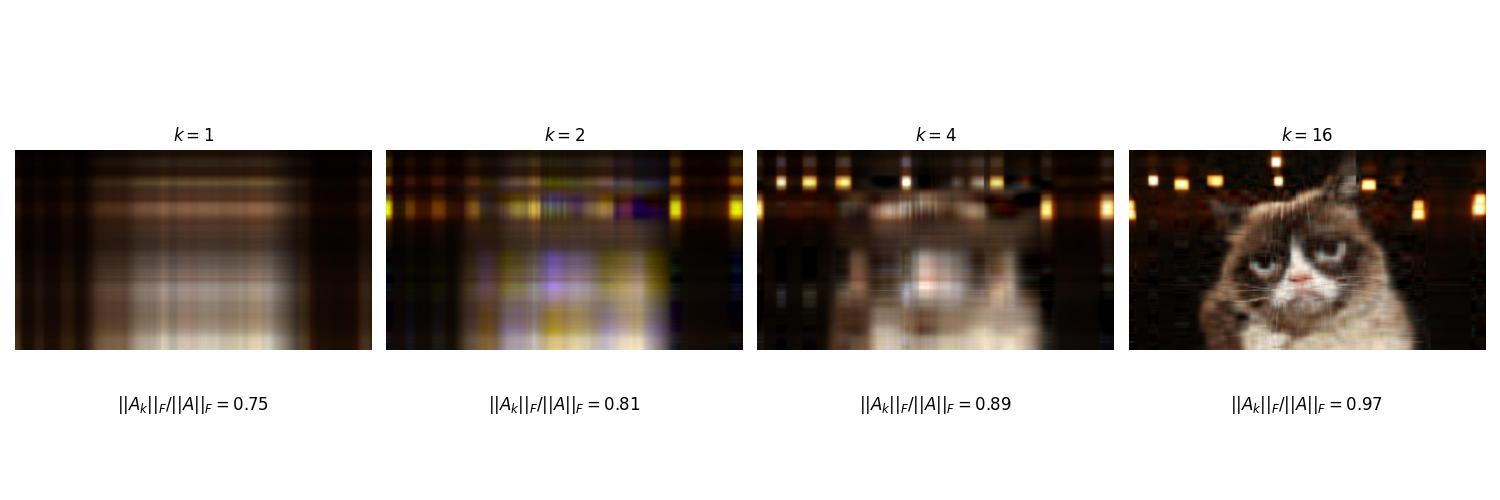
\includegraphics[scale=0.45]{/Users/nreef/Desktop/Spring_2025/CSE_382M/ps_2/hw2_code/grumpy_final.jpg}
  \caption{Exercise 3.28 Grumpy Cat Image}
\end{figure}

  \lstinputlisting[breaklines,language=Python]{/Users/nreef/Desktop/Spring_2025/CSE_382M/ps_2/hw2_code/image_convert.py}

\section*{Problem 2}
Below is the code,
\lstinputlisting[breaklines,language=Python]{/Users/nreef/Desktop/Spring_2025/CSE_382M/ps_2/hw2_code/h2q2.py}
Where the metric used is the $l_2$ norm of the means. The results are as follows.
\begin{figure}[H]
\centering
  \begin{tabular}{c|c|c|c}
    \toprule
    d & sep & err & err_k \\ \hline{}
    \midrule
    128 & 2.800000 & 7833.715623 & 7530.961809 \\
    128 & 4.800000 & 12910.938768 & 12727.029125 \\
    128 & 8.800000 & 23276.776722 & 23842.659448 \\
    64 & 0.800000 & 407.226630 & 519.826968 \\
    64 & 2.800000 & 1515.458966 & 1661.103212 \\
    64 & 4.800000 & 2866.817932 & 2833.834689 \\
    64 & 8.800000 & 5078.749828 & 5125.914381 \\
    16 & 0.800000 & 24.355424 & 19.554686 \\
    16 & 2.800000 & 73.194710 & 62.157570 \\
    16 & 4.800000 & 123.091010 & 150.093613 \\
    16 & 8.800000 & 223.719214 & 217.659231 \\
    8 & 0.800000 & 3.620507 & 7.620087 \\
    8 & 2.800000 & 9.540235 & 16.193273 \\
    8 & 4.800000 & 16.244131 & 16.254271 \\
    8 & 8.800000 & 50.563351 & 71.443154 \\
    \bottomrule
  \end{tabular}
\end{figure}
l
for $k=d/2$ and where \texttt{err} is the standard $l_2$ error between the $\mu_i$ using the normal dataset, while \texttt{err\_k} is the $l_2$ error after using the truncated SVD for the best projection of $X$ onto $k$-dimensional subspace. 

\section*{Problem 3}
Consider the matricies $B \in \R^{m \times n}$ and $C \in \R^{k \times l}$ that are fixed. Let $X \in \R^{n \times k}$ be such that the entries are i.i.d. with expectation $0$ and variance $1$. Then we see that
\begin{equation*}
  \norm{BXC}_F^2 = \tr(C^TX^TB^TBXC) 
\end{equation*}
and hence the expectation is given by
\begin{equation*}
  \EX{\norm{BXC}_F^2} = \Tr(C^T\EX{X^TB^TBX}C) = \Tr(C^T\EX{X^TX}B^TBC) = \Tr(C^TB^TBC) = \norm{BC}_F^2 = \norm{B}_F^2\norm{C}_F^2
\end{equation*}
\section*{Problem 4}
\lstinputlisting[breaklines,language=Python]{/Users/nreef/Desktop/Spring_2025/CSE_382M/ps_2/hw2_code/h2q4.py}

\begin{figure}[H]
  \centering
  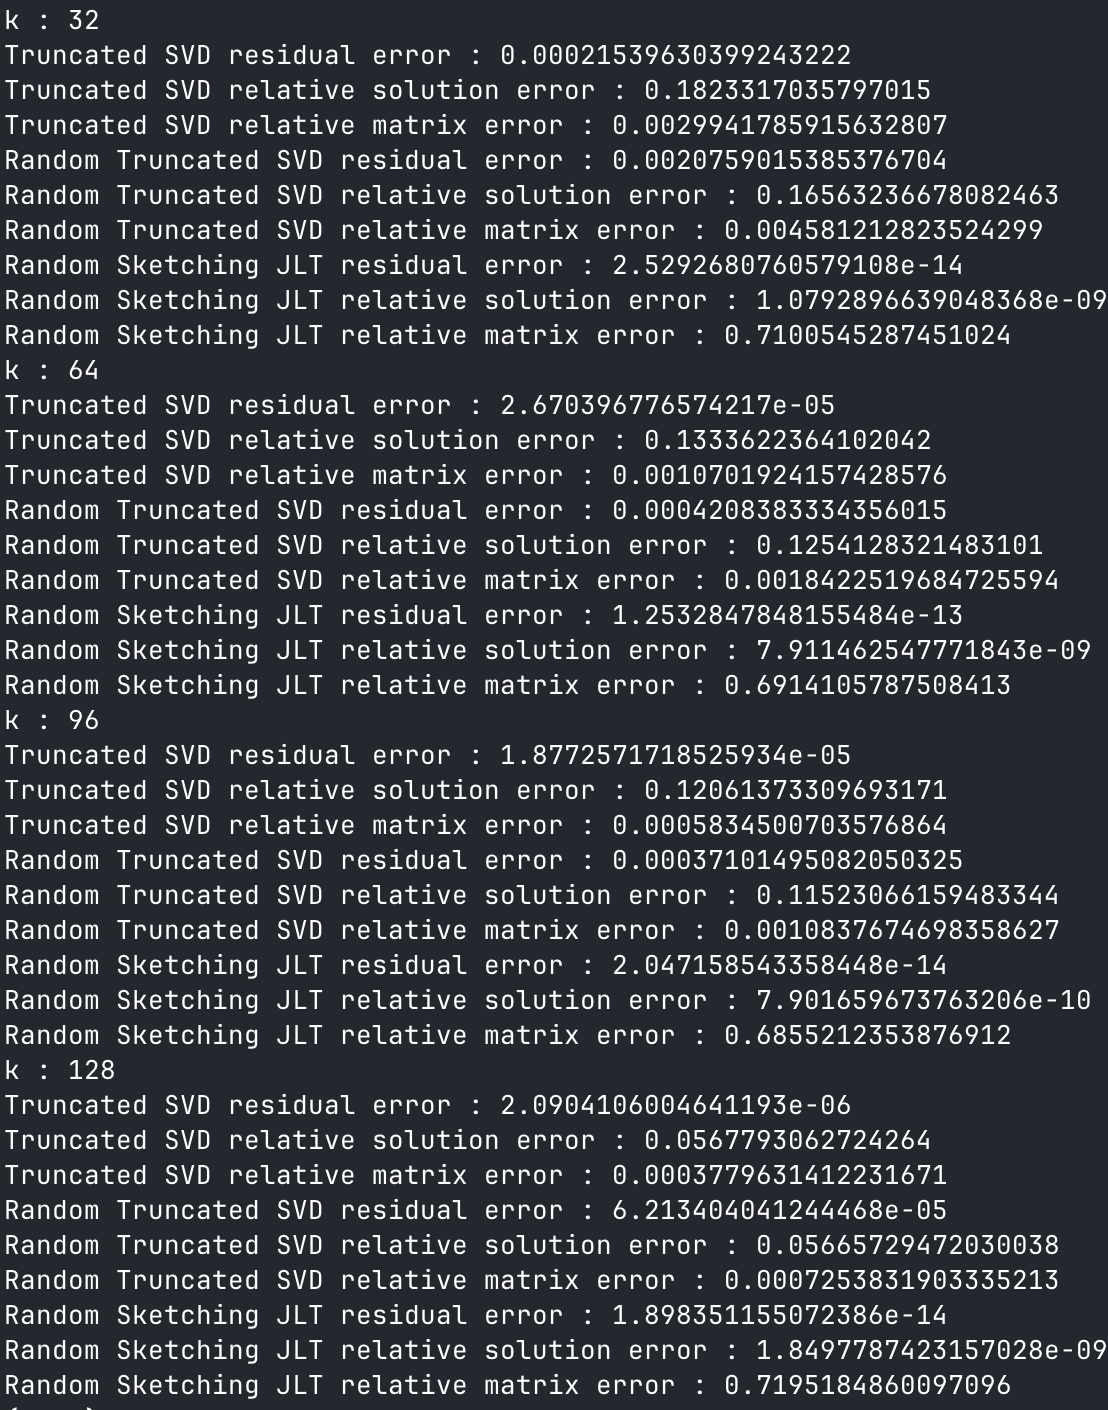
\includegraphics[scale=0.55]{/Users/nreef/Desktop/Spring_2025/CSE_382M/ps_2/hw2_code/results.png}
  \caption{Code Results}
\end{figure}
 
For the matrix error of each method, we have that for Truncated SVD that the expected error is given by
\begin{equation*}
  \frac{\norm{A - A_k}_2}{\norm{A}_2} - \frac{\sigma_{k+1}}{\sigma_1}
\end{equation*}
which in the case for $k = 32$ we get that the theoreitcal error is $\approx 0.0009$ 
for randomized SVD we have that for a $2k$ factorization that the expected error is given by
\begin{equation*}
  \EX{\norm{A - A_k}_2} = O(1 + 9\sqrt{kn}) \sigma_{k+1}
\end{equation*}

\end{document}
